\section{Podobné aplikace}
Vývoj nástroje MT-ComparEval byl v určitých oblastech inspirován nástroji,
  které už mohou vývojáři běžně využívat při své práci.
Z těchto nástrojů jsme se snažili vybrat ty nejdůležitější vlastnosti,
  které jsme později zkombinovali do jednoho funkčního celku.
V následující části budou tyto nástroje podrobněji představeny.

\subsection{mteval-11b.pl}
Je skript napsaný v jazyce Perl,
  který umožňuje počítat metriky BLEU a NIST.
Tento skript je celosvětově používaný,
  a proto byl použit pro kontrolu,
  že metriku BLEU v MT-ComparEval počítáme správně.

V současné době už existuje verze mteval-13a.pl,
  v které mimojiné přibyla možnost počítat metriky pro jednotlivé segmenty v překladu.
Postup, který k tomu použila je dále analyzován v kapitole Metriky strojového překladu.

\subsection{iBLEU}
\begin{figure}[h]
  \center
  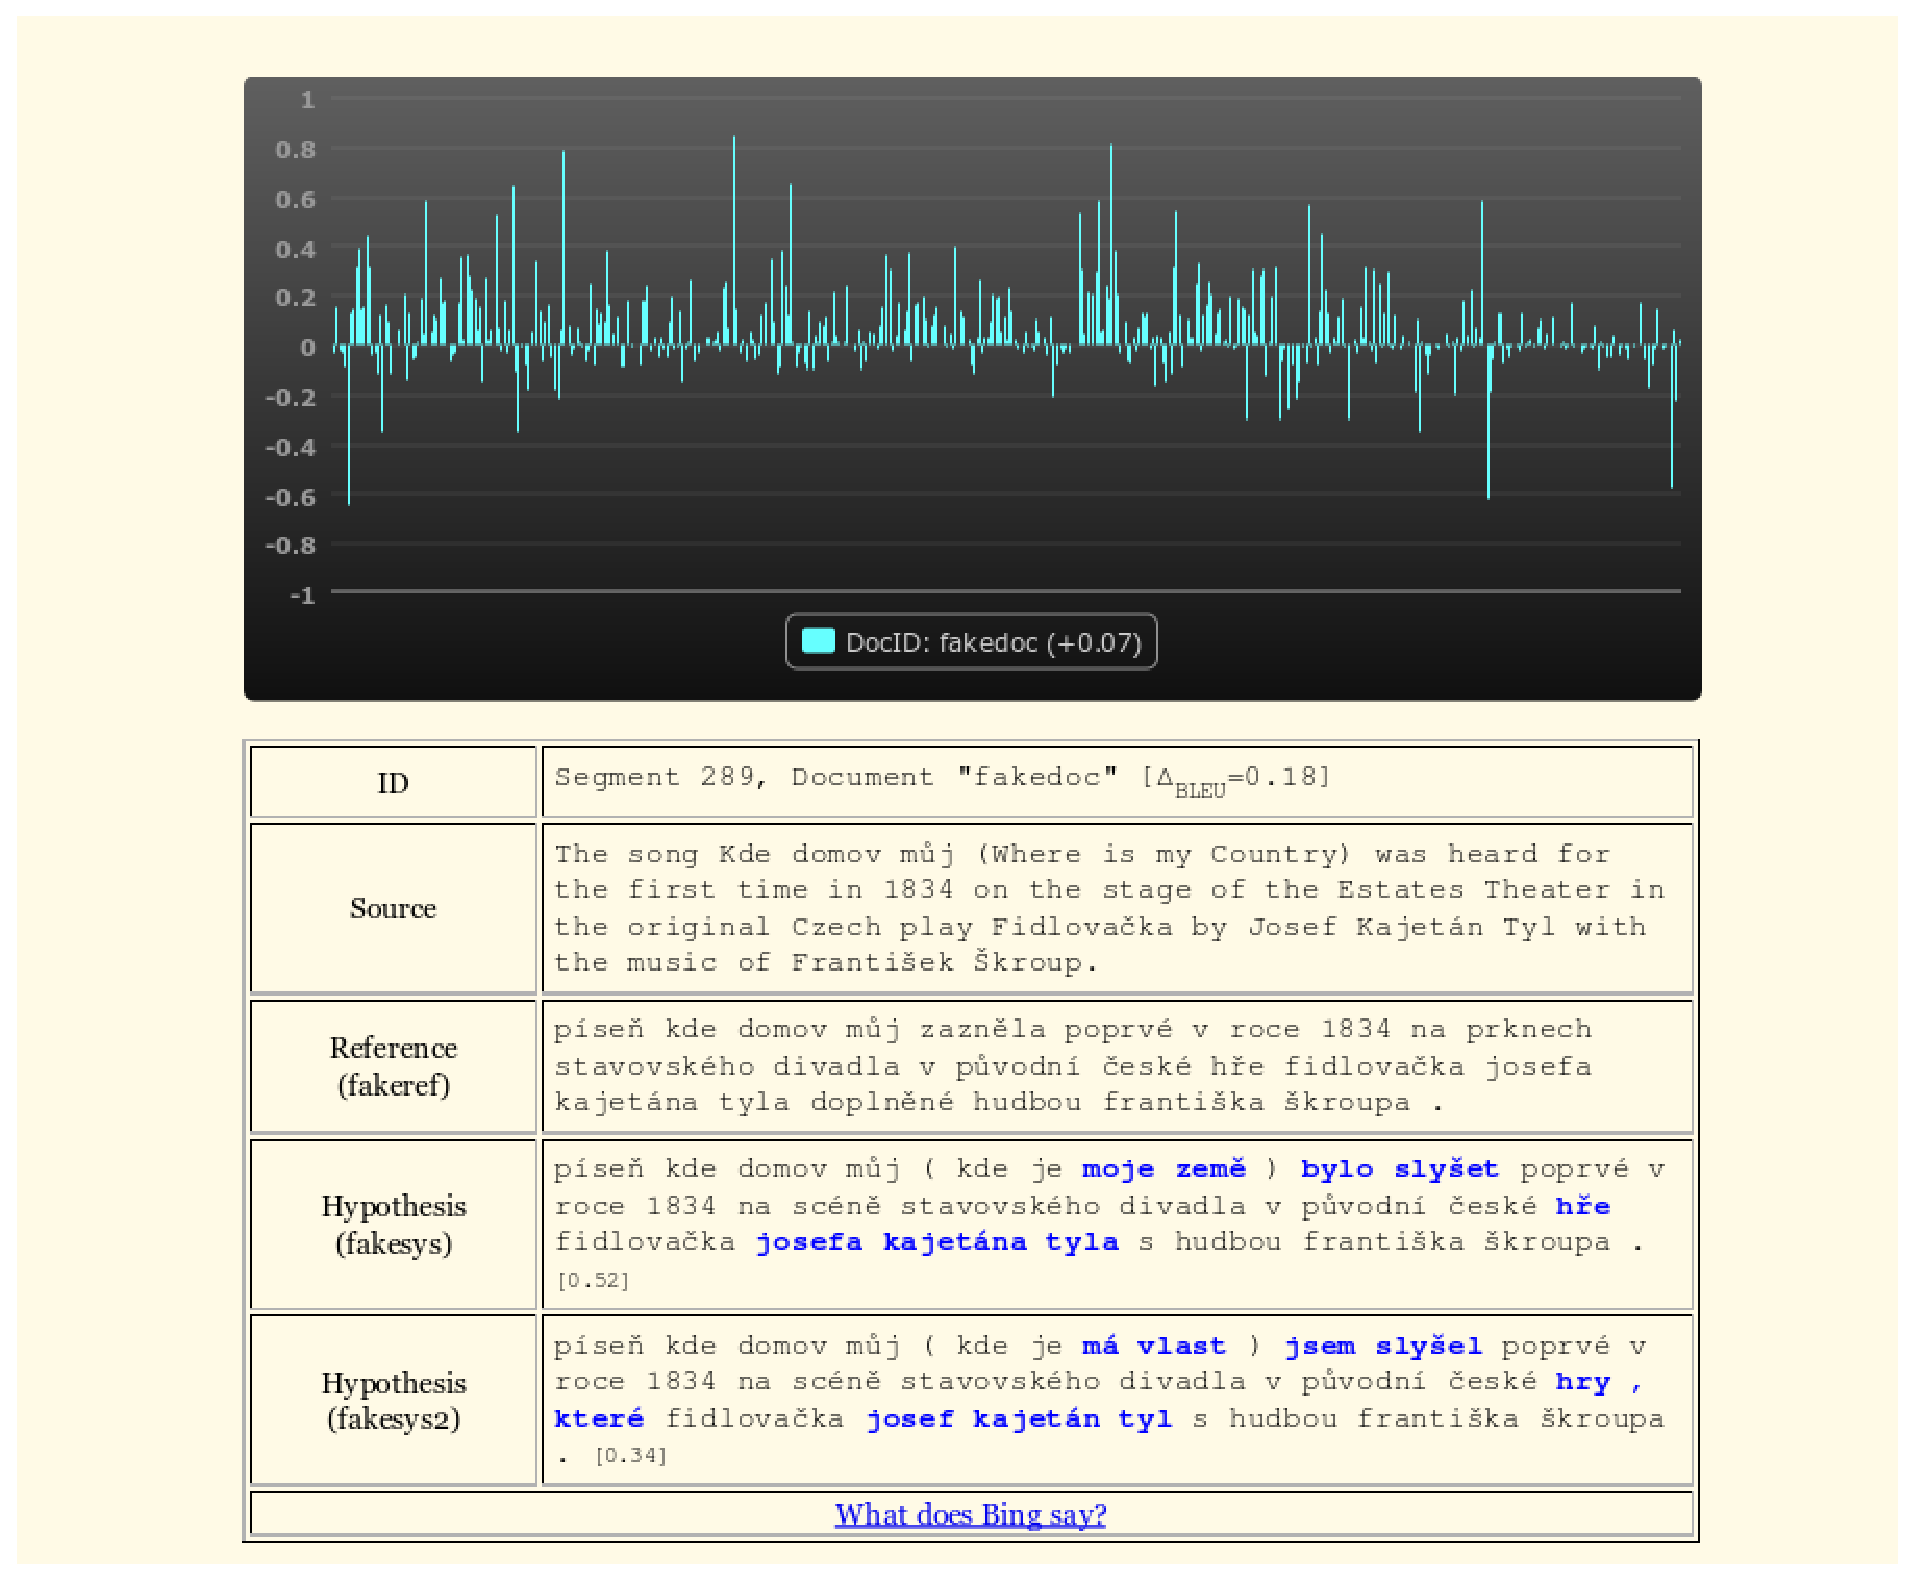
\includegraphics[width=0.9\textwidth]{img/ibleu.eps}
\end{figure}
Nástroj iBLEU umožňuje vyhodnocovat a porovnávat strojové překlady.
Pokud uživatel nemá žadný jiný strojový překlad,
  s kterým by chtěl svůj překlad porovnat,
  může si větu nechat přeložit překladačem Google Translate nebo Bing Translator
  a porovnat svůj překlad s překladem z tohoto nástroje.
Bohužel Google Translate nenabízí bezplatné api.
Bing Translator nabízí bezplatné api do limitu 2 miliónů přeložených znaků za den.
Pomocí tohoto nástroje můžeme počítat BLEU pro celé dokumenty nebo i jednotlivé segmenty
  a podle jejich výsledku si je můžeme později prohléhnout.

Pokud uživatel porovnává svůj strojový překlad pouze s referenčním překladem,
  je zvýrazněn jejich diff.
V případě, že uživatel porovnává dva strojové překlady,
  je zobrazen diff těchto překladů.

Tento nástroj je možné používat lokálně jako webovou aplikaci bez použití webového serveru,
  protože je celý napsán v HTML 5, CSS a javascriptu.
Stejně jako MT-ComparEval i iBLEU používá pro počítání BLEU jako referenční implementaci mteval-13a.pl.

\subsection{EMS - An Experimental Management System}
